\chapter{WF-140 Respecting the Dojo Ratchet To 1729}\label{record-222}

\noindent{\footnotesize\color{BookMuted}\path{docs/design/WF-140-respecting-dojo-ratchet-1729.md}\par}\smallskip

\section{Status}\label{record-222-status}

Implemented.

\section{Issue}\label{record-222-issue}

\begin{itemize}
\tightlist
\item
  GitHub Issue: \href{https://github.com/flyingrobots/bijou/issues/385}{\#385}
\end{itemize}

\section{Context}\label{record-222-context}

WF-139 landed the Respecting the Dojo burndown at \texttt{1\allowbreak{},\allowbreak{}7\allowbreak{}7\allowbreak{}9} aggregate Code Dojo violations. The next ratchet must cut at least \texttt{5\allowbreak{}0} more violations and set the ceiling to \texttt{1\allowbreak{},\allowbreak{}7\allowbreak{}2\allowbreak{}9} or lower.

The goal remains zero ESLint findings, zero Code Dojo warnings/errors/issues, and zero length-restriction violations. This cycle is one real cleanup slice toward that endpoint, not an exception shuffle.

\section{Goal}\label{record-222-goal}

Reduce aggregate Code Dojo debt from \texttt{1\allowbreak{},\allowbreak{}7\allowbreak{}7\allowbreak{}9} to \texttt{1\allowbreak{},\allowbreak{}7\allowbreak{}2\allowbreak{}9} or lower by eliminating at least \texttt{5\allowbreak{}0} live ESLint findings with behavior-preserving TypeScript fixes.

\section{Final Slice}\label{record-222-final-slice}

The implemented cleanup removes exactly 50 live ESLint findings:

\begin{center}
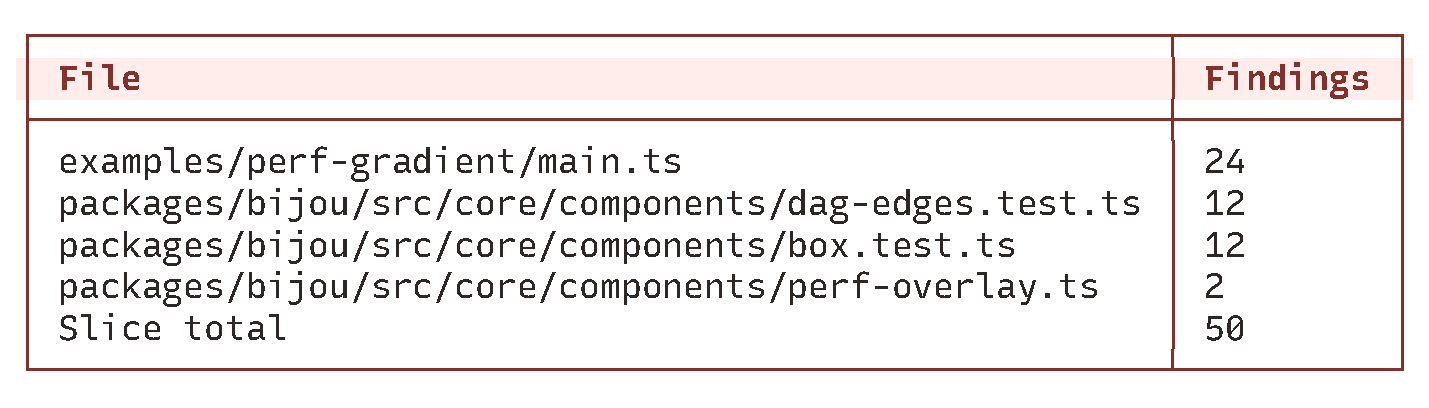
\includegraphics[width=\linewidth]{figures/tables/table-050-g1-1.pdf}
\par\smallskip{\scriptsize\color{BookMuted}Rows 1–5. Actual Bijou table component.}
\end{center}


The DOGFOOD capture candidate is intentionally deferred because touching that source currently activates a broader DOGFOOD i18n raw-copy cleanup than this goalpost should carry.

\section{Scope}\label{record-222-scope}

\begin{itemize}
\tightlist
\item
  Replace non-null assertions, unsafe assertions, and \texttt{a\allowbreak{}n\allowbreak{}y} escapes with checked reads, typed helpers, or narrowed runtime guards.
\item
  Make numeric and unknown template interpolation explicit.
\item
  Preserve perf-gradient and component behavior.
\item
  Lower \texttt{s\allowbreak{}c\allowbreak{}r\allowbreak{}i\allowbreak{}p\allowbreak{}t\allowbreak{}s\allowbreak{}/\allowbreak{}c\allowbreak{}o\allowbreak{}d\allowbreak{}e\allowbreak{}-\allowbreak{}d\allowbreak{}o\allowbreak{}j\allowbreak{}o\allowbreak{}/\allowbreak{}b\allowbreak{}a\allowbreak{}s\allowbreak{}e\allowbreak{}l\allowbreak{}i\allowbreak{}n\allowbreak{}e\allowbreak{}s\allowbreak{}/\allowbreak{}e\allowbreak{}s\allowbreak{}l\allowbreak{}i\allowbreak{}n\allowbreak{}t\allowbreak{}.\allowbreak{}j\allowbreak{}s\allowbreak{}o\allowbreak{}n}, \texttt{d\allowbreak{}o\allowbreak{}c\allowbreak{}s\allowbreak{}/\allowbreak{}c\allowbreak{}o\allowbreak{}d\allowbreak{}e\allowbreak{}-\allowbreak{}d\allowbreak{}o\allowbreak{}j\allowbreak{}o\allowbreak{}-\allowbreak{}e\allowbreak{}x\allowbreak{}c\allowbreak{}e\allowbreak{}p\allowbreak{}t\allowbreak{}i\allowbreak{}o\allowbreak{}n\allowbreak{}s\allowbreak{}.\allowbreak{}m\allowbreak{}d}, and \texttt{p\allowbreak{}a\allowbreak{}c\allowbreak{}k\allowbreak{}a\allowbreak{}g\allowbreak{}e\allowbreak{}.\allowbreak{}j\allowbreak{}s\allowbreak{}o\allowbreak{}n} only after live counts prove the reduction.
\end{itemize}

\section{Non-Goals}\label{record-222-non-goals}

\begin{itemize}
\tightlist
\item
  ESLint rules, Code Dojo thresholds, and standards artifacts must not weaken.
\item
  File/context and code-size ceilings must not rise.
\item
  Broad DOGFOOD architecture rewrites are out of scope.
\item
  Exception churn cannot stand in for real cleanup.
\end{itemize}

\section{Current Evidence}\label{record-222-current-evidence}

Live counts on \texttt{m\allowbreak{}a\allowbreak{}i\allowbreak{}n} at \texttt{7\allowbreak{}e\allowbreak{}0\allowbreak{}2\allowbreak{}9\allowbreak{}d\allowbreak{}f\allowbreak{}7}:

\begin{itemize}
\tightlist
\item
  aggregate Code Dojo debt: \texttt{1\allowbreak{},\allowbreak{}7\allowbreak{}7\allowbreak{}9}
\item
  ESLint findings: \texttt{1\allowbreak{},\allowbreak{}3\allowbreak{}6\allowbreak{}8}
\item
  file/context baseline: \texttt{3\allowbreak{}3\allowbreak{}3}
\item
  mock-ban baseline: \texttt{2\allowbreak{}3}
\item
  code-size baseline: \texttt{5\allowbreak{}5}, including \texttt{4} legacy hard-limit files
\item
  next aggregate target: \texttt{1\allowbreak{},\allowbreak{}7\allowbreak{}2\allowbreak{}9} or lower
\end{itemize}

Implementation result:

\begin{itemize}
\tightlist
\item
  aggregate Code Dojo debt: \texttt{1\allowbreak{},\allowbreak{}7\allowbreak{}2\allowbreak{}9}
\item
  ESLint findings: \texttt{1\allowbreak{},\allowbreak{}3\allowbreak{}1\allowbreak{}8}
\item
  live ESLint reduction: \texttt{5\allowbreak{}0}
\item
  next aggregate target: \texttt{1\allowbreak{},\allowbreak{}6\allowbreak{}7\allowbreak{}9} or lower
\end{itemize}

\section{Playback Questions}\label{record-222-playback-questions}

\begin{enumerate}
\def\labelenumi{\arabic{enumi}.}
\tightlist
\item
  Is aggregate Code Dojo debt at \texttt{1\allowbreak{},\allowbreak{}7\allowbreak{}2\allowbreak{}9} or lower?
\item
  Did the implementation remove at least \texttt{5\allowbreak{}0} real violations?
\item
  Did touched file/context and code-size ceilings stay flat or lower?
\item
  Did focused behavior tests for touched surfaces pass?
\end{enumerate}

\section{Validation Plan}\label{record-222-validation-plan}

\begin{itemize}
\tightlist
\item
  Run focused Code Dojo gates for the touched files.
\item
  Run focused tests for the selected component surfaces.
\item
  Run \texttt{n\allowbreak{}p\allowbreak{}m\allowbreak{} \allowbreak{}r\allowbreak{}u\allowbreak{}n\allowbreak{} \allowbreak{}c\allowbreak{}o\allowbreak{}d\allowbreak{}e\allowbreak{}-\allowbreak{}d\allowbreak{}o\allowbreak{}j\allowbreak{}o\allowbreak{}:\allowbreak{}d\allowbreak{}e\allowbreak{}b\allowbreak{}t}.
\item
  Run \texttt{n\allowbreak{}p\allowbreak{}m\allowbreak{} \allowbreak{}r\allowbreak{}u\allowbreak{}n\allowbreak{} \allowbreak{}c\allowbreak{}o\allowbreak{}d\allowbreak{}e\allowbreak{}-\allowbreak{}d\allowbreak{}o\allowbreak{}j\allowbreak{}o\allowbreak{}:\allowbreak{}v\allowbreak{}e\allowbreak{}r\allowbreak{}i\allowbreak{}f\allowbreak{}y}.
\item
  Run \texttt{n\allowbreak{}p\allowbreak{}m\allowbreak{} \allowbreak{}r\allowbreak{}u\allowbreak{}n\allowbreak{} \allowbreak{}l\allowbreak{}i\allowbreak{}n\allowbreak{}t} and \texttt{n\allowbreak{}p\allowbreak{}m\allowbreak{} \allowbreak{}r\allowbreak{}u\allowbreak{}n\allowbreak{} \allowbreak{}l\allowbreak{}i\allowbreak{}n\allowbreak{}t\allowbreak{}:\allowbreak{}e\allowbreak{}s\allowbreak{}l\allowbreak{}i\allowbreak{}n\allowbreak{}t}.
\end{itemize}

\section{Acceptance Criteria}\label{record-222-acceptance-criteria}

\begin{itemize}
\tightlist
\item
  The selected touched TypeScript files have zero new ESLint findings and reduce live findings by at least \texttt{5\allowbreak{}0}.
\item
  Aggregate Code Dojo debt is \texttt{1\allowbreak{},\allowbreak{}7\allowbreak{}2\allowbreak{}9} or lower.
\item
  \texttt{s\allowbreak{}c\allowbreak{}r\allowbreak{}i\allowbreak{}p\allowbreak{}t\allowbreak{}s\allowbreak{}/\allowbreak{}c\allowbreak{}o\allowbreak{}d\allowbreak{}e\allowbreak{}-\allowbreak{}d\allowbreak{}o\allowbreak{}j\allowbreak{}o\allowbreak{}/\allowbreak{}b\allowbreak{}a\allowbreak{}s\allowbreak{}e\allowbreak{}l\allowbreak{}i\allowbreak{}n\allowbreak{}e\allowbreak{}s\allowbreak{}/\allowbreak{}e\allowbreak{}s\allowbreak{}l\allowbreak{}i\allowbreak{}n\allowbreak{}t\allowbreak{}.\allowbreak{}j\allowbreak{}s\allowbreak{}o\allowbreak{}n} records the lower live ESLint count.
\item
  \texttt{d\allowbreak{}o\allowbreak{}c\allowbreak{}s\allowbreak{}/\allowbreak{}c\allowbreak{}o\allowbreak{}d\allowbreak{}e\allowbreak{}-\allowbreak{}d\allowbreak{}o\allowbreak{}j\allowbreak{}o\allowbreak{}-\allowbreak{}e\allowbreak{}x\allowbreak{}c\allowbreak{}e\allowbreak{}p\allowbreak{}t\allowbreak{}i\allowbreak{}o\allowbreak{}n\allowbreak{}s\allowbreak{}.\allowbreak{}m\allowbreak{}d} and \texttt{p\allowbreak{}a\allowbreak{}c\allowbreak{}k\allowbreak{}a\allowbreak{}g\allowbreak{}e\allowbreak{}.\allowbreak{}j\allowbreak{}s\allowbreak{}o\allowbreak{}n} report the lower ceiling.
\item
  Focused validation for the touched surfaces passes.
\end{itemize}

